\documentclass[a4paper]{article}
\usepackage[utf8]{vietnam}
\usepackage[left=3.5cm,right=2.5cm,top=2cm,bottom=2cm]{geometry} 
\setlength{\parindent}{0pt}
\usepackage{graphicx} 
%\usepackage[firstpage]{draftwatermark} 
\usepackage{xcolor}
\usepackage{tikz} 
\usepackage{scrextend}
\changefontsizes{14pt}
%\usepackage{background}
\usetikzlibrary{calc}
\usepackage{listings}
\usepackage{pdfpages}

%\backgroundsetup{scale = 1, angle = 0, opacity = 0.2,
%contents = {\includegraphics[width = 0.9\paperwidth,
%height = 0.9\paperheight, keepaspectratio] {hust.png}}}

%\backgroundsetup{scale = 1, angle = 0, opacity = 0.2,
%contents = {
\includegraphics[width = 0.97\paperwidth,
%height = 0.97\paperheight, keepaspectratio] {bia.png}}}
\begin{document}
\begin{titlepage}
    %\SetWatermarkText{
\includegraphics[width = 0.97\paperwidth,
    %height = 0.97\paperheight]{bia.png}}
    %\SetWatermarkAngle{0} 
    %\SetWatermarkText{\includegraphics[scale=1]{hust.png}}
    %\SetWatermarkAngle{0} 
    \begin{tikzpicture}[remember picture,overlay,inner sep=0,outer sep=0]
        \draw[blue!70!black,line width=4pt] ([xshift=-1.5cm,yshift=-2cm]current page.north east) coordinate (A)--([xshift=1.5cm,yshift=-2cm]current page.north west) coordinate(B)--([xshift=1.5cm,yshift=2cm]current page.south west) coordinate (C)--([xshift=-1.5cm,yshift=2cm]current page.south east) coordinate(D)--cycle;

        \draw ([yshift=0.5cm,xshift=-0.5cm]A)-- ([yshift=0.5cm,xshift=0.5cm]B)--
        ([yshift=-0.5cm,xshift=0.5cm]B) --([yshift=-0.5cm,xshift=-0.5cm]B)--([yshift=0.5cm,xshift=-0.5cm]C)--([yshift=0.5cm,xshift=0.5cm]C)--([yshift=-0.5cm,xshift=0.5cm]C)-- ([yshift=-0.5cm,xshift=-0.5cm]D)--([yshift=0.5cm,xshift=-0.5cm]D)--([yshift=0.5cm,xshift=0.5cm]D)--([yshift=-0.5cm,xshift=0.5cm]A)--([yshift=-0.5cm,xshift=-0.5cm]A)--([yshift=0.5cm,xshift=-0.5cm]A);


        \draw ([yshift=-0.3cm,xshift=0.3cm]A)-- ([yshift=-0.3cm,xshift=-0.3cm]B)--
        ([yshift=0.3cm,xshift=-0.3cm]B) --([yshift=0.3cm,xshift=0.3cm]B)--([yshift=-0.3cm,xshift=0.3cm]C)--([yshift=-0.3cm,xshift=-0.3cm]C)--([yshift=0.3cm,xshift=-0.3cm]C)-- ([yshift=0.3cm,xshift=0.3cm]D)--([yshift=-0.3cm,xshift=0.3cm]D)--([yshift=-0.3cm,xshift=-0.3cm]D)--([yshift=0.3cm,xshift=-0.3cm]A)--([yshift=0.3cm,xshift=0.3cm]A)--([yshift=-0.3cm,xshift=0.3cm]A);

    \end{tikzpicture}
    \begin{center}
        \vspace{7pt}

        \textbf{ĐẠI HỌC BÁCH KHOA HÀ NỘI}

        \vspace{7pt}
        {\fontsize{13pt}{9.6pt}\selectfont\textbf{TRƯỜNG CÔNG NGHỆ THÔNG TIN \& TRUYỀN THÔNG}}
    \end{center}
    \vspace{10pt}
    \begin{center}
        
\includegraphics[scale=0.4]{HUST_SOICT.png}

        \vspace{30pt}
        \fontsize{18pt}{17pt}\selectfont
        \textbf{BÁO CÁO}

        \vspace{7pt}
        \textbf{ Mini-Project}
    \end{center}
    \begin{flushleft}
        \fontsize{14pt}{17pt}\selectfont
        \textbf{\textsl{ĐỀ TÀI}}
        \vspace{7pt}
    \end{flushleft}
    \begin{center}
        \fontsize{18pt}{17pt}\selectfont
        \textbf{INTRODUCTION TO }

        \vspace{7pt}
        \textbf{COMMUNICATION ENGINEERING}
    \end{center}

    \vspace{15pt}
    \textbf{Giảng viên hướng dẫn: PhD. Trịnh Văn Chiến}

    \vspace{10pt}
    \textbf{Nhóm sinh viên thực hiện:}

    \begin{tabbing}
        \hspace{8cm}\=\hspace{3cm}\=\hspace{3cm} \kill
        {\it \textbf{Họ và tên}}\>{\it \textbf{MSSV}}\>{\it \textbf{Mã lớp}}\\
         \begin{bfseries}Phan Trung Dũng (1)\end{bfseries}\> \begin{bfseries}20205073\end{bfseries}\> \begin{bfseries}135279\end{bfseries}\\
        \begin{bfseries}Hoàng Minh Ngọc (2)\end{bfseries}\> \begin{bfseries}20200440\end{bfseries}\> \begin{bfseries}135279\end{bfseries}\\
        \begin{bfseries}Hoàng Vân Trường (3)\end{bfseries}\> \begin{bfseries}20205134\end{bfseries}\> \begin{bfseries}135279\end{bfseries}\\
    \end{tabbing}
    \vspace{10pt}
    \begin{center}
        \textbf{Hà Nội, 2023}
    \end{center}
\end{titlepage}
\newpage
\begin{center}
    \fontsize{30pt}{17pt}\selectfont
        \textbf{Mục Lục}
\end{center}
\renewcommand\contentsname{}
\tableofcontents
\newpage
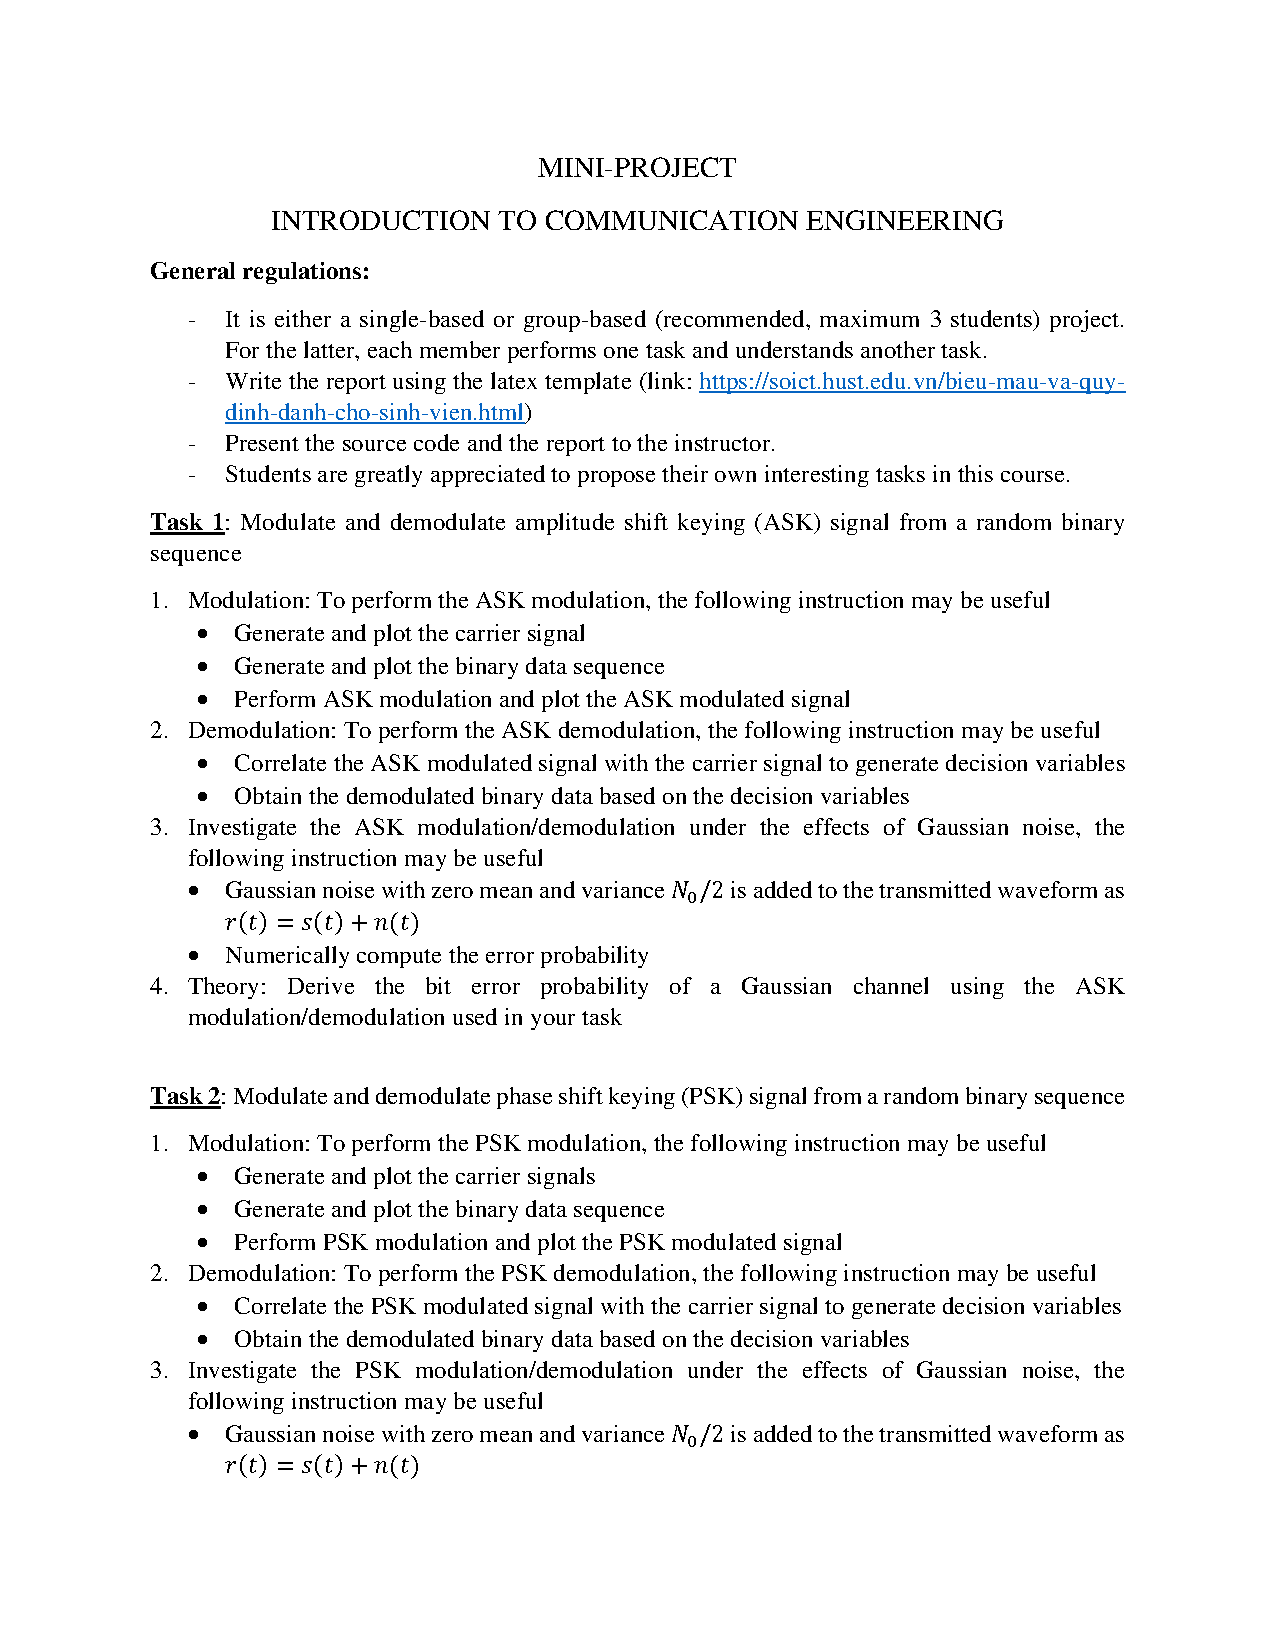
\includepdf[pages=-]{MiniProject.pdf}
\newpage
\begin{center}
    \fontsize{30pt}{17pt}\selectfont
        \textbf{Lời cảm ơn}
\end{center}
Sau khi đào sâu tìm hiểu, cũng như tự hệ thống lại kiến thức để có thể thực hiện
Mini Project này, em tự thấy bản thân đã học học được thêm rất nhiều kiến thức
mới, hiểu kỹ và sâu sắc hơn những công thức trên lý thuyết được học.
Em cũng rất mong thời gian tới sẽ có cơ hội được tiếp xúc, thực hành nhiều hơn
với các hệ thống truyền thông để chúng em có thể hiểu được áp dụng triệt để những
lý thuyết đã học ở trường.
\\
em xin trân thành cảm ơn thầy Trịnh Văn Chiến đã cho chúng em được làm bài, hệ thống lại kiến thức vô cùng bổ ích của môn học Kỹ Thuyết Truyền Thông, bọn em thấy bài học khá là hay và thú vị, rất là ý nghĩa trong chương trình học của bọn em, em mong muốn có thể gặp thầy trong những bài học, học phần hấp dẫn tới. \\
chúng em xin chân thành cảm ơn.
\newpage

\section{Điều chế và giải điều chế ASK (Amplitude Shift Keying)}
\label{section:1}
\subsection{Không gian tín hiệu 2-ASK:}
\label{subsection:1.1}
ASK (Binary Amplitude Shift Keying) là một loại kỹ thuật điều chế biên độ số. Tín hiệu ASK có dạng sóng giao động tần số f, sóng tín hiệu truyền đi được tạo ra bằng cách thay đổi biên độ của sóng mang.\\

\begin{center}
    \begin{figure}[htp]
    \begin{center}
     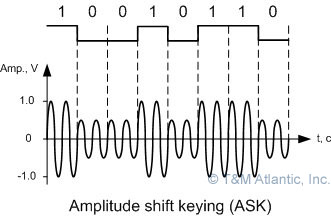
\includegraphics[]{Img/keying_ASK}
    \end{center}
    \label{refhinh1}
    \end{figure}
\end{center}

Trong điều chế 2-ASK, một bit sẽ được gán với một sóng mang với biên độ khác nhau.\\
Không gian tín hiệu 2-ASK:
\begin{center}
\begin{equation*}
   $ M = \{s_{1} = A_{1}sin(2\pi ft) ; s_{2} = A_{2}sin(2\pi ft)\} $
\end{equation*}
\end{center}
Cơ sở trực chuẩn: $b(t) = \sqrt{\frac{2}{T}}sin(2\pi ft)$ với $T = \frac{1}{R_{b}}$.
\subsection{Kênh tạp âm trắng có tính cộng AWGN}
Ở mọi hệ thống truyền thông, tín hiệu nhận được đều bị méo đi do có nhiễu. Ở đây, ta giả thiết nhiễu là nhiễu Gauss trắng có tính cộng. \\
Kênh AWGN có các tính chất sau:
\begin{itemize}
    \item Tuyến tính và bất biến theo thời gian
    \item Đáp ứng tần số lý tưởng $H(f) = 1$
    \item Tạp âm Gaus có tính cộng 
    \begin{itemize}
        \item Tiến trình ngẫu nhiên ergodic: các đặc trưng thống kê của tiến trình có thể suy ra được từ một chuỗi các mẫu đủ dài của nó
        \item Mỗi biến ngẫu nhiên tuân theo phân phối chuẩn Gauss với giá trị trung bình bằng 0
    \end{itemize}
    \item Mật độ công suất phổ tín hiệu là hằng số $G_{n}(f) = \frac{N_{0}}{2}$
    
\end{itemize}

\subsection{Bộ lọc phối hợp (Matched Filter)}
Chọn bộ lọc có đáp ứng xung $h(t) = b(T-t)$ ta được bộ lọc phối hợp.\\
Tín hiệu đầu vào bộ lọc là tín hiệu nhận được bên bộ thu: $\rho (t)$. \\
Đáp ứng xung là: $h(t) = b_{j}(t)$ \\
Đầu ra của bộ lọc phối hợp là: 
\begin{center}
    $y(t) = \int_{-\infty}^{+\infty} \rho(\tau)h(t-\tau)\  dx = \int_{-\infty}^{+\infty} \rho(\tau)b_{j}(T-t+\tau)\  dt$
\end{center}
Giả thiết lấy mẫu tín hiệu đầu ra tại thời điểm $T = 1$:
\begin{center}
    $y(t=T) = \int_{-\infty}^{+\infty} \rho(\tau)b_{j}(\tau)\  dx = \int_{0}^{T} \rho(\tau)b_{j}(\tau)\  d\tau$
\end{center}
Như vậy, sử dụng MF cho ta một phương án thay thế có thể được dùng để tính toán các phép chiếu $b_{j}(t)$ thay vì phải sử dụng các bộ tích phân các bộ tích phân
\begin{center}
    \begin{figure}[htp]
    \begin{center}
     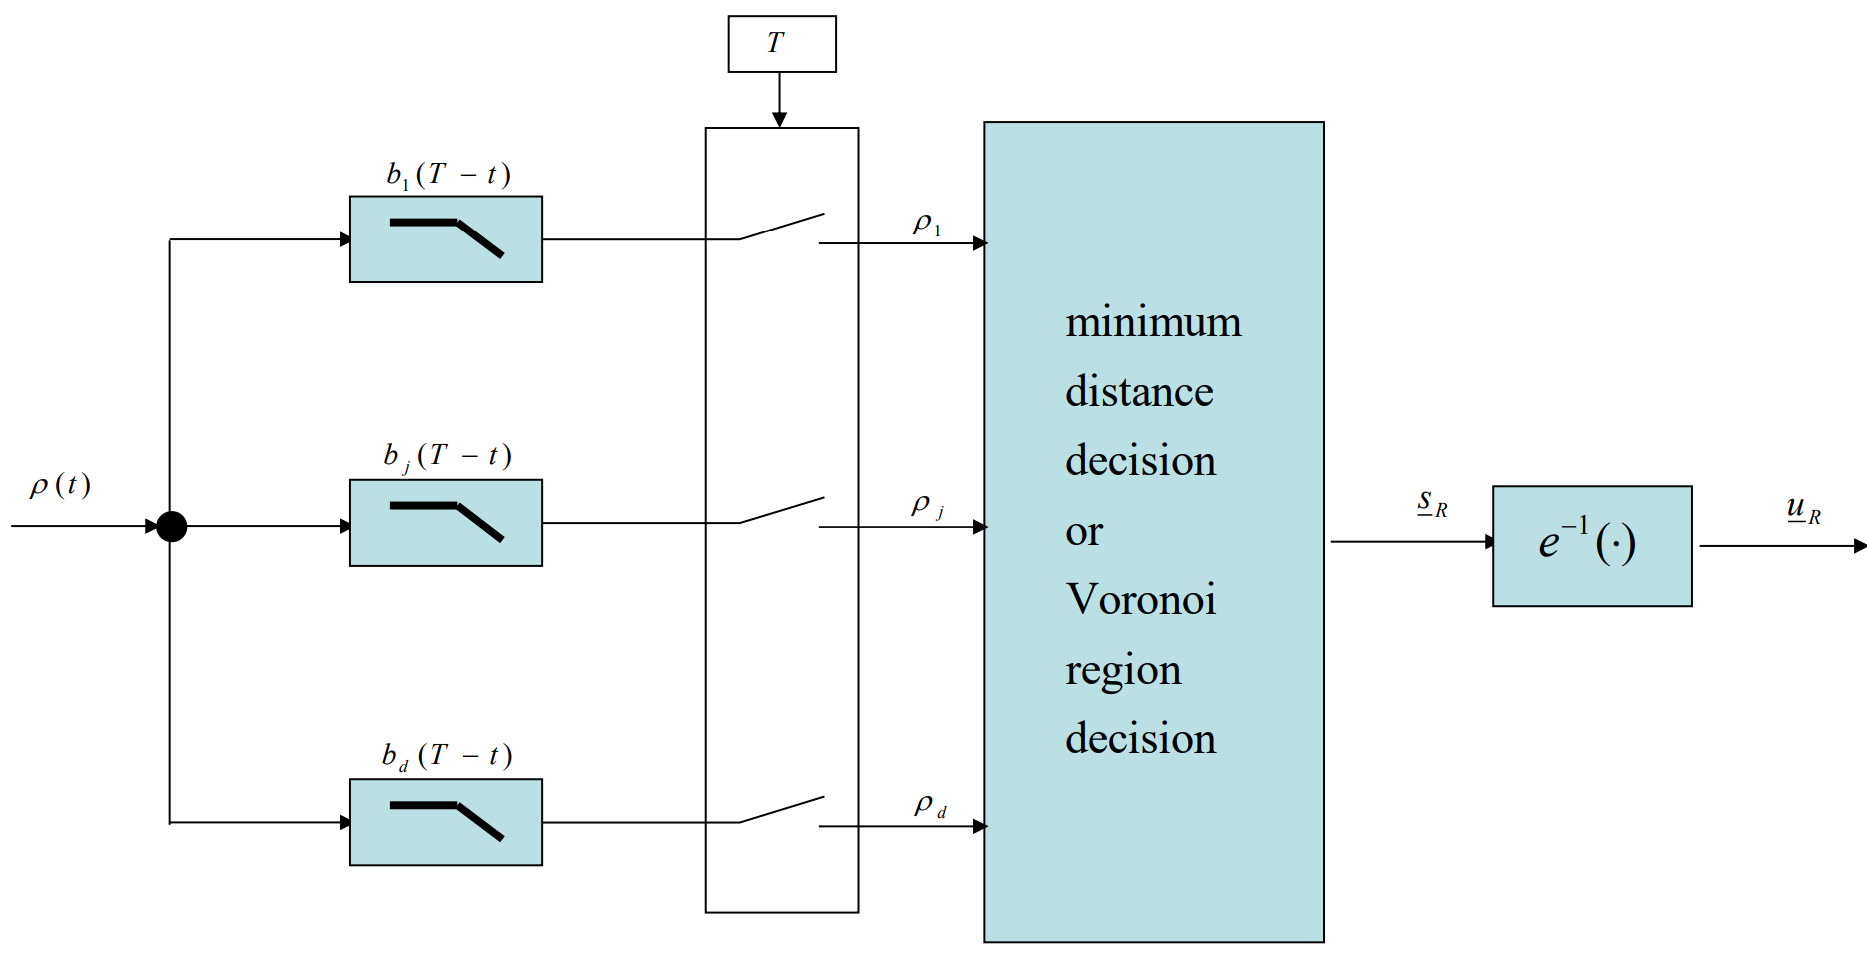
\includegraphics[width=\textwidth]{Img/MF.png}
    \end{center}
    \end{figure}
\end{center}
\newpage
\subsection{Giải thích Code}
Đầu tiên ta khai báo các thư viện để tính toán và mô phỏng các tín hiệu:
\begin{lstlisting}
import random
import numpy as np
import matplotlib.pyplot as plt
import math
\end{lstlisting}
Số lượng bit truyền đi: 8
Thời gian truyền 1 bit: 1
Thời gian truyền tín hiệu: 8
Tạo mạng bit ngẫu nhiên:
\begin{lstlisting}
N = 8      
Tb = 1     
T = 1*N    
t = np.arange(0, Tb, Tb/800)
def random_bits_array(n): 
    return [random.randint(0, 1) for _ in range(n)]
m = random_bits_array(N)
\end{lstlisting}
\textbf{Điều chế 2-ASK} \\
Chuyển các bit thành các tín hiệu tương ứng: \\ 
\begin{itemize}
    \item 1: $A_{1}sin(2\pi f t)$
    \item 0: $A_{2}sin(2\pi ft)$
\end{itemize}
Ta chọn $A_{1} = 1$ , $A_{2} = 0.25$ , $f = 2R_{b}$
\begin{lstlisting}
f = 2    
A1 = 1    
A2 = 0.25 
def modulation():
    out = []
    f = 2    
    A1 = 1    
    A2 = 0.25 
    t = np.arange(0, Tb, Tb/100)
    s1 = A1 * np.sin(2 * np.pi * f * t)
    s2 = A2 * np.sin(2 * np.pi * f * t)
    for i in range(len(m)):
        if m[i] == 0:
            out.extend(s2)
        if m[i] == 1:
            out.extend(s1)
    return out
ask = modulation()
\end{lstlisting}
Kết quả:\\
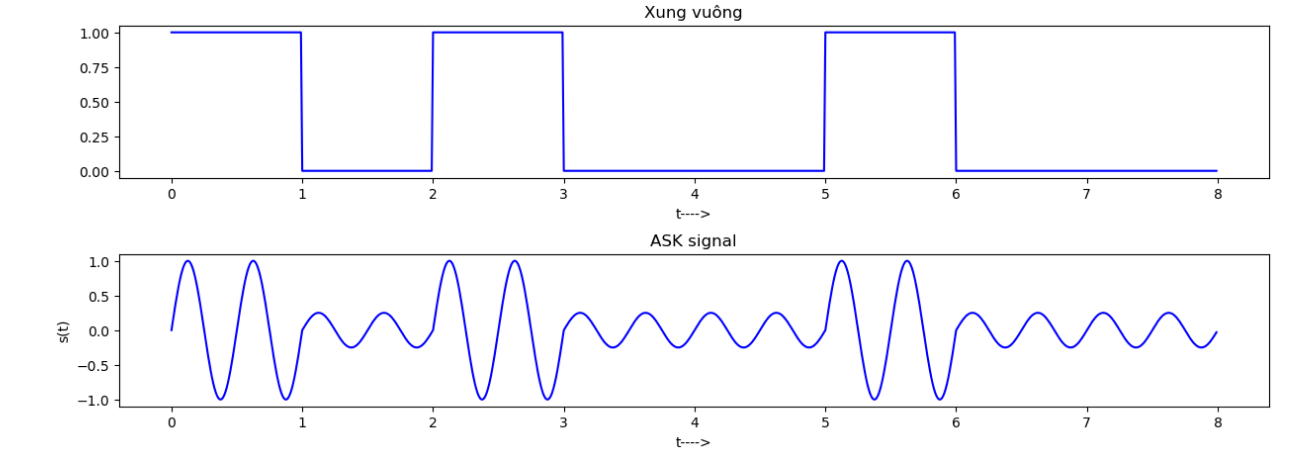
\includegraphics[width=\textwidth]{Img/ASK_f.png}
\\
\textbf{Thêm nhiễu Gauss} \\ 
Nhiễu Gauss được thêm vào có giá trị trung bình là 0, phương sai $\frac{N_{0}}{2}$
\begin{lstlisting}
N0 = 0.1
noise = np.random.normal(0, np.sqrt(N0/2), len(ask)) 
ask_noisy = ask + noise
\end{lstlisting}
Kết quả: \\
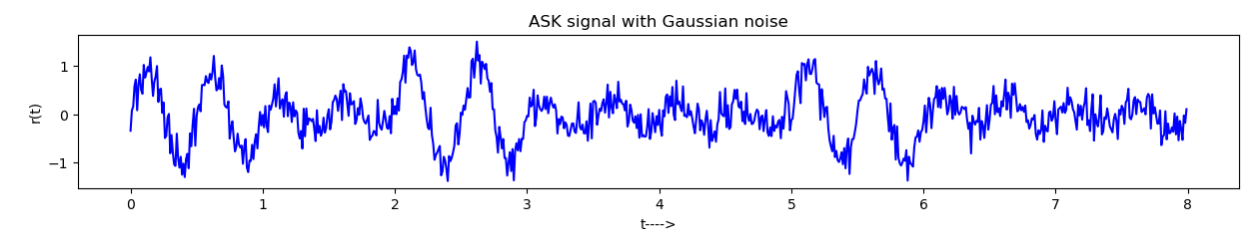
\includegraphics[width=\textwidth]{Img/ASK_N.png}
\textbf{Giải điều chế tín hiệu}\\
Cách làm: Ta tính hình chiếu của tín hiệu $r(t)$ trên cơ sơ trực chuẩn $B$ , sau đó ra quyết định bằng tiêu chuẩn khoảng cách ngắn nhất để khôi phục tín hiệu $s(t)$ ở nơi nhận. \\
Cơ sở trực chuẩn $B = \{b(t) = \sqrt{\frac{2}{T_{b}}}sin(2\pi ft)\}$\\
Sử dụng bộ lọc phối hợp tính các hình chiếu của $r(t)$ lên không gian trực chuẩn $M$:\\
$\rho[n] = \int_{nT_{b}}^{(n+1)T_{b}} \rho(t)b_{j}(t)\  dt $ \\
Áp dụng tiêu chuẩn khoảng cách nhỏ nhất ta suy ra:\\
Nếu $\rho[n] \geq \sqrt{\frac{T_{b}}{2}}\frac{(A_{1}+A_{2})}{2} $, ký tự nhị phân khôi phục $s'[n] = 1$.\\
Nếu $\rho[n] < \sqrt{\frac{T_{b}}{2}}\frac{(A_{1}+A_{2})}{2} $, ký tự nhị phân khôi phục $s'[n] = 0$.\\
Source code:
\begin{lstlisting}
def demodulation():
    t = np.arange(0, Tb, Tb/100)
    hx = math.sqrt(2/Tb)*np.sin(2 * np.pi * f * t)
    ask_noisy_list = np.array_split(ask_noisy, 8)
    output = []
    for i in range(len(ask_noisy_list)):
        if np.trapz(ask_noisy_list[i] * hx,t) >= np.sqrt(Tb
/2)*(A1+A2)/2:
            output.append(1)
        else:
            output.append(0)
    return output

demod = demodulation()
\end{lstlisting}
Kết quả: \\
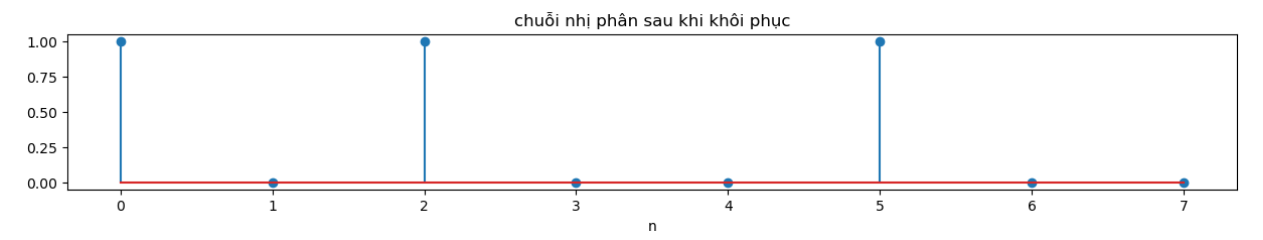
\includegraphics[width=\textwidth]{Img/In_Signal.png}
\subsection{Xác xuất lỗi:}
Ta đã có kết luận: Các không gian tín hiệu khác nhau (khác dạng sóng truyền) nhưng có cùng không gian vector thì có BER như nhau.\\
Do đó $BER = SER = \frac{1}{2}erfc(\sqrt{\frac{E_{0}}{N_{0}}})$

\newpage

\section{Điều chế và Giải điều chế PSK (Phase Shift Keying)}
\subsection{Giới thiệu về PSK}
PSK là sơ đồ điều chế kỹ thuật số truyền dữ liệu bằng cách thay đổi hoặc điều chế
pha của tín hiệu tham chiếu (sóng mang). PSK sử dụng một số giai đoạn hữu hạn, mỗi
giai đoạn được gán một mẫu chữ số nhị phân duy nhất. Thông thường, mỗi pha mã hóa
một số bit bằng nhau. Mỗi mẫu bit định dạng biểu tượng được biểu thị bằng pha cụ thể. \\
Trong hệ thống điều chế BPSK, tín hiệu băng tần gốc được gắn vào sóng mang bằng
cách thay đổi pha của sóng mang tùy thuộc vào tín hiệu băng gốc. \\
Giả sử có sóng mang được biểu diễn: \\
 $ x_{0}(t) = A.\sin(\omega_{0} + \varphi) $\\
Biểu thức tín hiệu gốc: S(t) là tín hiệu nhị phân (0,1) hay là chuỗi NRZ. \\ 
Do đó ta có: \\ 
- Khi $ s(t) = 0: P(t) = A.sin(\omega_{0}) $ \\
- Khi $ s(t) = 0: P(t) = A.sin(\omega_{0} + \pi) $ \\ 

Đối với khóa dịch pha PSK, thông tin chứa trong pha tức thời của sóng mang điều chế.
Thường thì pha này được ấn định và so sánh tương thích với sóng mang của pha đã biết
- PSK kết hợp. Kiểu điều chế BPSK này còn được gọi là điều chế khóa đảo pha PRK
(Phase Reversal Keying). Hình 7.7, trình bày bộ phát PRK, dạng sóng tín hiệu và phổ.
\begin{center}
     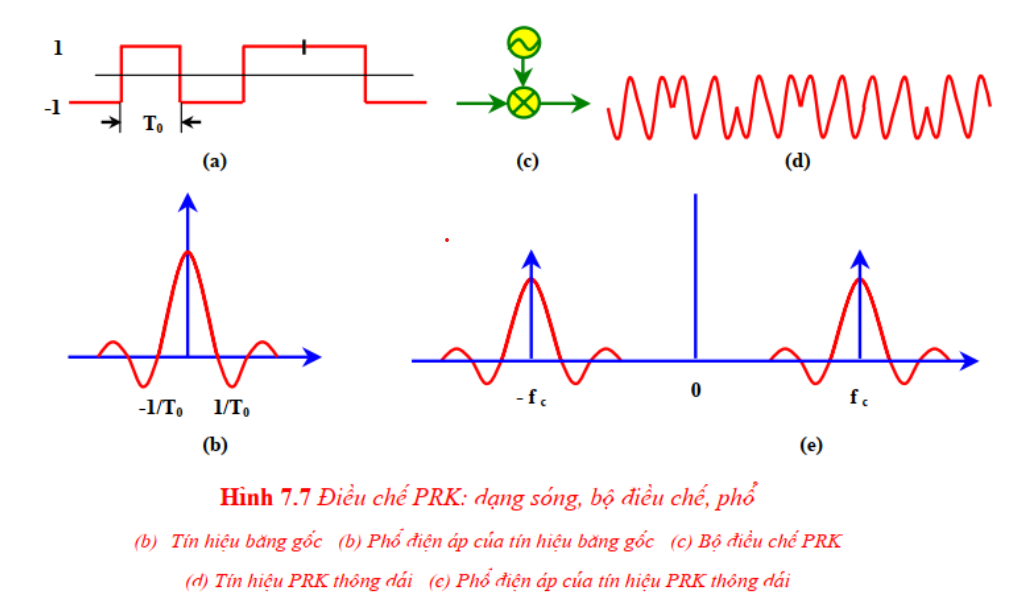
\includegraphics[scale=.5]{Img/dieuchepho.png}
\end{center}
\subsection{Nguyên tắc khóa dịch pha nhị phân}
Nguyên tắc : Các tín hiệu nhị phân tác dụng lên sóng mang làm thay đổi pha của
sóng mang. Cụ thể là: \\ 
• Bit 1: pha của sóng mang là 0. \\ 
• Bit 0: pha của sóng mang là $ 180^{o}.$\\  
Bảng chân lý của tín hiệu điều chế BPSK:
\begin{center}
     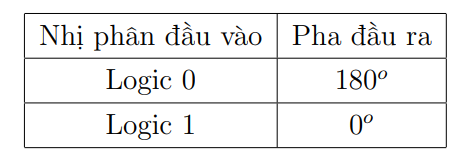
\includegraphics[scale=.5]{Img/bangchanlyPSK.png}
\end{center}
Có thể thấy rõ hơn trong cách biểu diễn trên đồ thị thời gian và trạng thái của tín
hiệu BPSK.
\begin{center}
     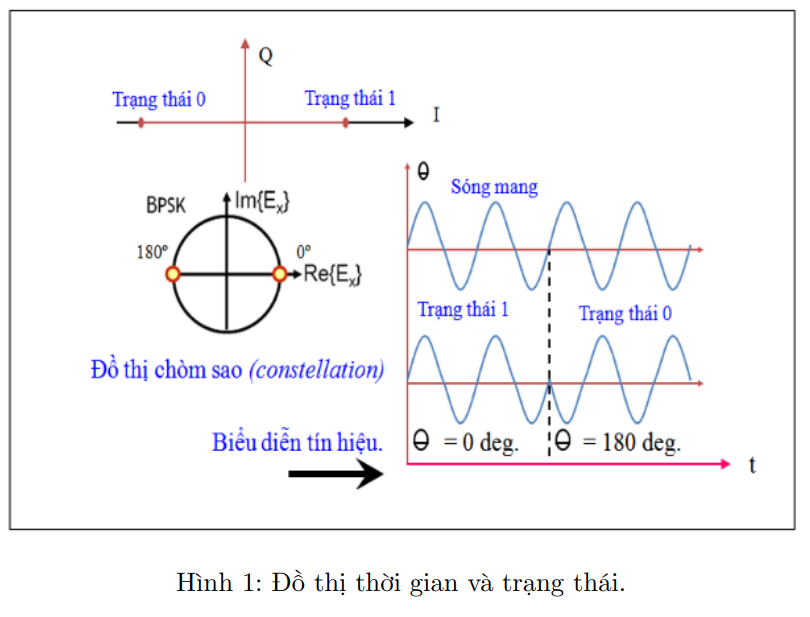
\includegraphics[scale=.7]{Img/bangtrangthai.png}
\end{center}
\subsection{Điều chế PSK}
\begin{center}
     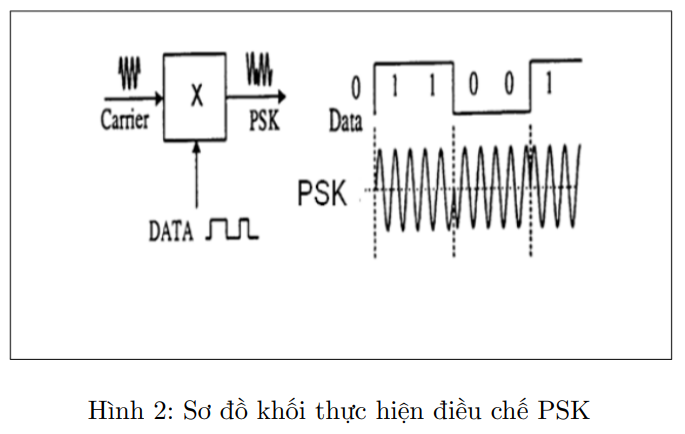
\includegraphics[scale=.7]{Img/sododieuchePSK.png}
\end{center}
Phương pháp điều chế 2-PSK hay BPSK (Binary PSK) hay điều chế ngược pha (Phase
Reversal Keying) được giới thiệu ở hình trên. \\ Sơ đồ tạo tín hiệu BPSK dạng sin với hai giá trị pha tùy thuộc vào giá trị Data: \\ 
- Khi data bit = 1, tín hiệu BPSK cùng pha với sóng mang \\ 
- Khi data bit = 0, tín hiệu BPSK ngược pha ($180^{o}$) với sóng mang. \\ 
\begin{center}
     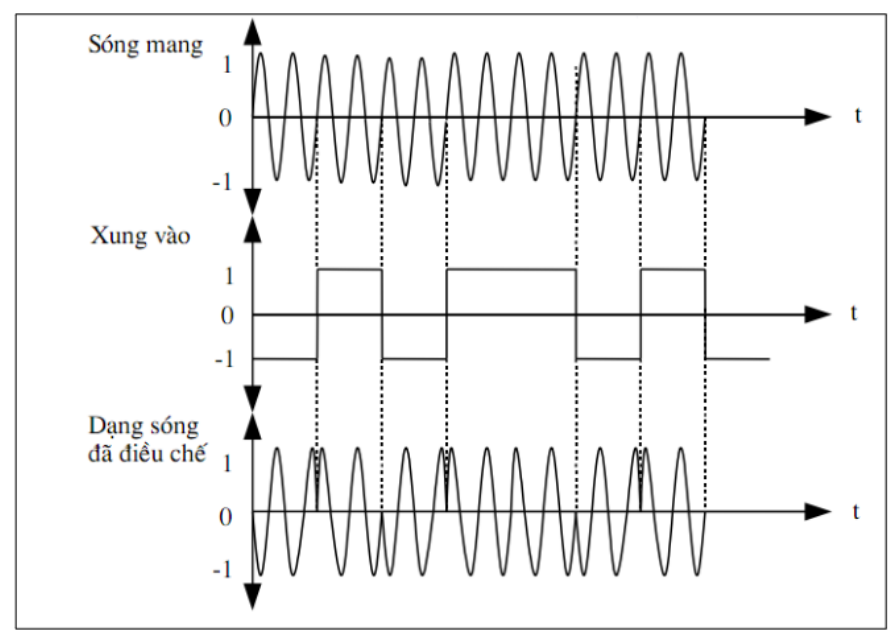
\includegraphics[scale=.5]{Img/quanhethoigiandieuche.png} \\ 
     Hình 3: Quan hệ pha/thời gian \\  ở đầu ra bộ điều chế PSK theo tín hiệu vào
\end{center}  \\
\newpage
\textbf{Mô hình điều chế PSk}
\begin{center}
    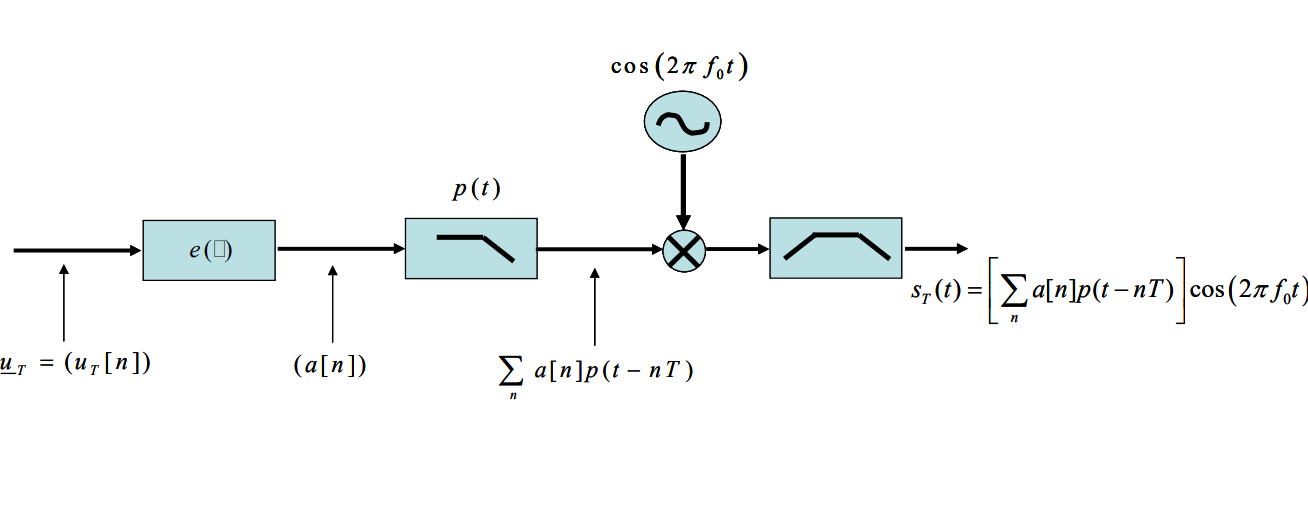
\includegraphics[scale=.6]{Img/bieudoASK.png}
\end{center}
\begin{center}
    \textbf{Mô hình điều chế PSK}
\end{center}

\newpage
\subsection{Mã nguồn điều chế tín hiệu PSK sử dụng ngôn ngữ Python, trình bày Jupyter Notebook }
\\ 
\textbf{ - Thêm thư viện} \\
import random \\ 
import numpy as np \\
import matplotlib.pyplot as plt \\ 
from scipy.signal import butter, filtfilt \\ 
\textbf{hàm tạo mảng bit ngẫu nhiên} \\ 
\begin{lstlisting}
def random_bits_array(n):   
    return [random.randint(0, 1) for _ in range(n)] 
\end{lstlisting}
\textbf{Hàm tạo tín hiệu xung vuông và xung vuông đảo ngược}
\begin{lstlisting}
def message_signal(m,T):                         
    t = np.arange(0, T, T/100)             
    message = []                           
    not_message = []
    for i in range(len(m)): 
        if m[i] == 1:                     
            m_s = np.ones(len(t))          
            invm_s = np.zeros(len(t))
        else:
            m_s = np.zeros(len(t))         
            invm_s = np.ones(len(t))       
        message.extend(m_s)                 
        not_message.extend(invm_s)         
    return message , not_message    
    
\end{lstlisting}
\textbf{khai báo}
\begin{lstlisting}
N = 8    
T = 1        
Tb = 1*N      
t = np.arange(0, Tb, Tb/800)  
m = random_bits_array(N) 
fc = 2                                         
songmang = np.sqrt(2/Tb) * np.sin(2 * np.pi * fc * t)  
\end{lstlisting}
\textbf{Vẽ sóng mang}
\begin{lstlisting}
fig, ax = plt.subplots(1, 1, figsize=(15, 2))   
fig.subplots_adjust(hspace=0.5)                 
ax.plot(t, c)                                  
ax.set_title('Tin hieu song mang')           
ax.set_xlabel('t --->')
ax.set_ylabel('c1(t) ---> ')
\end{lstlisting}
\begin{center}
     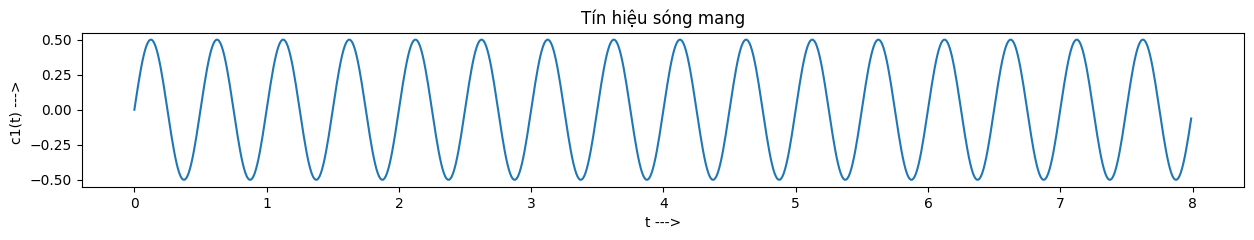
\includegraphics[scale=.5]{Img/tinhieusongmang.png}
\end{center}

\textbf{Vẽ chuỗi nhị phân và xung vuông tương ứng}
\begin{lstlisting}
fig, ax = plt.subplots(2, 1, figsize=(15, 5))               
fig.subplots_adjust(hspace=0.5)                           
ax[0].stem(m)                                          
ax[0].set_title('Chuoi nhi phan sinh ngau nhien')
ax[0].set_xlabel('n -->')
ax[0].set_ylabel('b(n) --->')
message , not_message = message_signal(m,T)                
print(len(message), len(not_message))
ax[1].plot(t,message, 'r')                                 
ax[1].set_title('Tin hieu xung vuong')
ax[1].set_xlabel('t --->')
ax[1].set_ylabel('c1(t) --->')
\end{lstlisting}
\begin{center}
     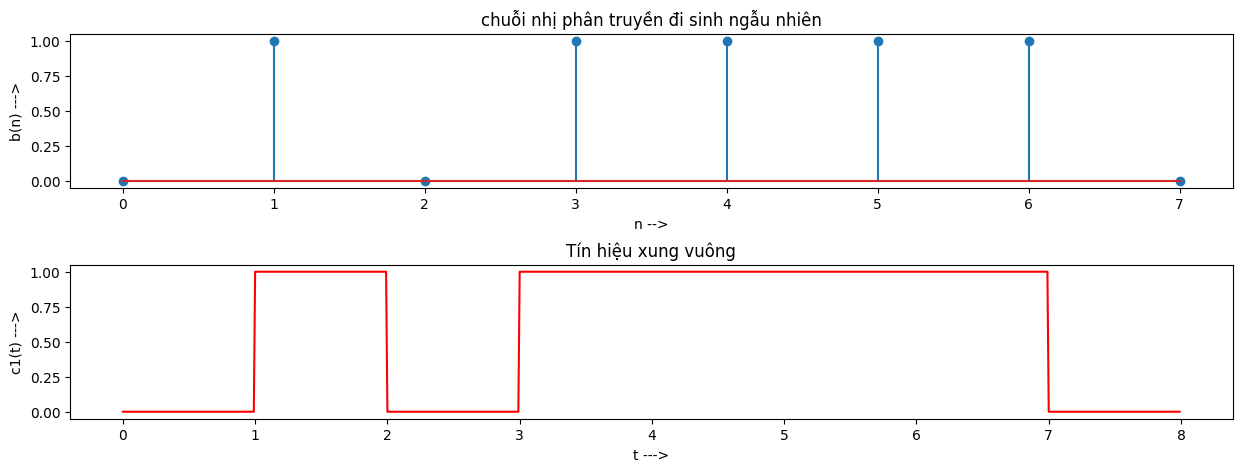
\includegraphics[scale=.5]{Img/vechuoinhiphantuognung.png}
\end{center}
\textbf{Điều chế PSK}
\begin{lstlisting}
def modulation(message_signal,not_message_signal):              
    return message_signal*songmang
            - not_message_signal*songmang  
psk = modulation(message,not_message)                              
\end{lstlisting}
\textbf{Tín hiệu PSK sau khi điều chế}
\begin{lstlisting}
fig, ax = plt.subplots(1, 1, figsize=(15, 2))    
ax.figsize=(15, 5)
ax.plot(t,psk, 'b')
ax.set_title('PSK signal')
ax.set_xlabel('t---->')
ax.set_ylabel('Gia tri')
\end{lstlisting}
\begin{center}
     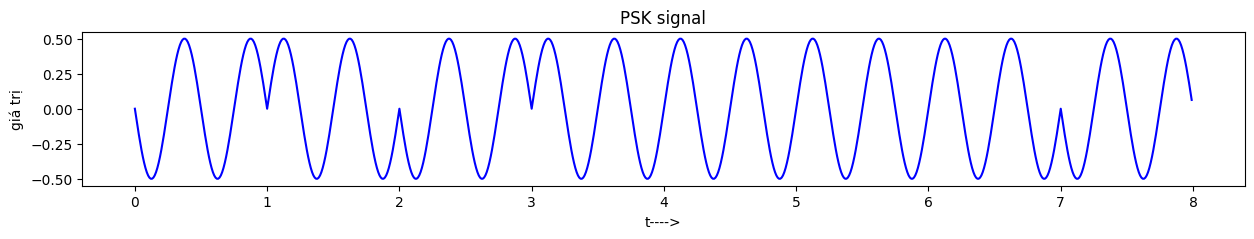
\includegraphics[scale=.5]{Img/tinhieuPSKsaukhidieuche.png}
\end{center}
\subsection{Giải điều chế PSK}
\textbf{Bộ giải điều chế BPSK bao gồm:} \\
- Sơ đồ lấy bình phương để chuyển các tín hiệu khác pha về cùng 1 pha \\ 
- Vòng giữ pha PLL phát lại nhịp với tần số gấp đôi tần số sóng mang \\ 
- Bộ chia pha $\Delta\phi$ để hiệu chỉnh pha \\ 
- Bộ chia hai để đưa tần số tín hiệu tái lập về bằng tần số sóng mang \\ 
- Bộ nhân tín hiệu thực hiện nhân sóng điều chế PSK với sóng mang tái lập \\ 
Giả sử tần số sóng mang là fc, $\omega$ c = 2$\pi$fc, ta có hai trường hợp: \\ 
Khi tín hiệu PSK là $+\sin(\omega_{c}t)$ ứng với Data bit = 1, sóng mang tái lập là $\sin(\omega_{c}t)$, sơ đồ nhân sẽ cho tín hiệu: \\
$\sin(\omega_{c}t).\sin(\omega_{c}t)) = \sin(\omega_{c}t)^{2}$
$ = \frac{1}{2}.(1 - \cos(2\omega_{c}t)) = \frac{1}{2} - \frac{1}{2} \cos(2.\omega_{c}t)$
Trong biểu thức trên, thành phần thứ hai là xoay chiều, có tần số gấp đôi tần số sóng mang. Khi sử dụng bộ lọc thông thấp với tần số cắt bằng tần số sóng mang, ta có thể khử bỏ thành phần xoay chiều và thế dương của thành phần một chiều thứ nhất được giữ lại sẽ biểu diễn trạng thái "1" của bit Data.

Khi tín hiệu PSK là $-\sin(\omega_{c}t)$ ứng với Data bit = 0,sơ đồ nhân sẽ cho tín hiệu \\
$-\sin(\omega_{c}t).\sin(\omega_{c}t)) = -\sin(\omega_{c}t)^{2}$
$ = -\frac{1}{2}.(1 - \cos(2\omega_{c}t)) = -\frac{1}{2} + \frac{1}{2} \cos(2.\omega_{c}t)$
Trong biểu thức trên, thành phần thứ hai là xoay chiều, có tần số gấp đôi tần số sóng mang. \textbf{Khi sử dụng bộ lọc thông thấp với tần số cắt bằng tần số sóng mang, ta có thể khử bỏ thành phần xoay chiều} và thế âm của thành phần một chiều thứ nhất được giữ lại sẽ biểu diễn trạng thái "0" của bit Data.
\subsection{Mã nguồn giải điều chế tín hiệu PSK sử dụng ngôn ngữ Python,
trình bày Jupyter Notebook}
\textbf{Hàm giải mã tín hiệu}
# Nếu tín hiệu mẫu trùng với sóng sin được sử dụng, thì tổng của tích sóng sẽ lớn, 
# còn nếu tín hiệu mẫu không trùng với sóng sin được sử dụng, tổng của tích sóng sẽ nhỏ.
# Để tính tổng này, chúng ta dùng vòng lặp để chạy qua mỗi giá trị của N, 
# tính tổng với khoảng tín hiệu tương ứng, rồi cập nhật giá trị start và end cho lần chạy tiếp theo của vòng lặp.
\begin{lstlisting}
    def demodulation(filtered_signal,N):                                # giải mã tín hiệu nhận được
    start = 0
    end = 100
    demod = np.zeros(N)
    for i in range(N):
        x = np.sum(songmang[start:end] 
                * filtered_signal[start:end])
        if x > 0:
            demod[i] = 1
        else:
            demod[i] = 0
        start += 100
        end += 100
    return demod
\end{lstlisting}
\textbf{Vẽ tín hiệu sau khi điều chế }
\begin{center}
     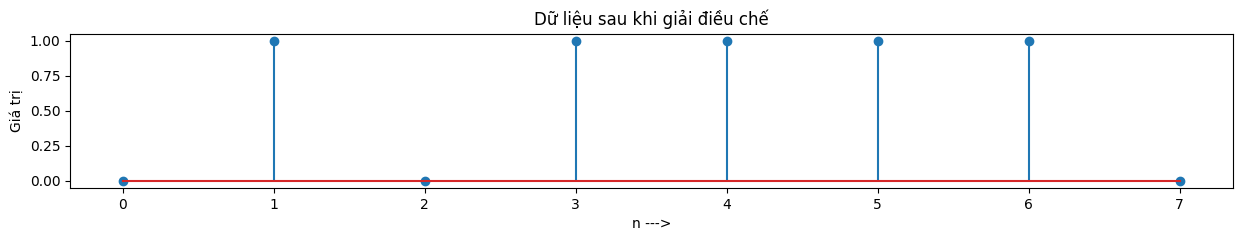
\includegraphics[scale=.5]{Img/dulieusaudieuche.png}
\end{center}
\newpage
\section{ Điều tra điều chế/giải điều chế PSK dưới tác động của nhiễu Gaussian }
Nhiễu Gaussian là một tín hiệu ngẫu nhiên có mật độ phân bố công suất phẳng nghĩa làtín hiệu nhiễu có công suất bằng nhau trong toàn khoảng băng thông. Tín hiệu này có tên là nhiễu trắng vì nó có tính chất tương tự với ánh sáng trắng. Chúng ta không thể tạo ra nhiễu trắng theo đúng lý thuyết vì theo định nghĩa của nó, nhiễu trắng có mật độ phổ công suất phân bố trong khoảng tần vô hạn và do vậy nó cũng phải có công suất vô hạn. Tuy nhiên, trong thực tế, chúng ta chỉ cần tạo ra nhiễu trắng trong khoảng băng tần của hệ thống chúng ta đang xem xét. \\ 
Với khóa dịch pha nhị phân (PSK), các bit nhị phân 1 và 0 có thể được biểu thị
bằng các mức năng lượng tương ứng : $+\sqrt{E_{b} $ và $-\sqrt{E_{b} $.
\begin{center}
     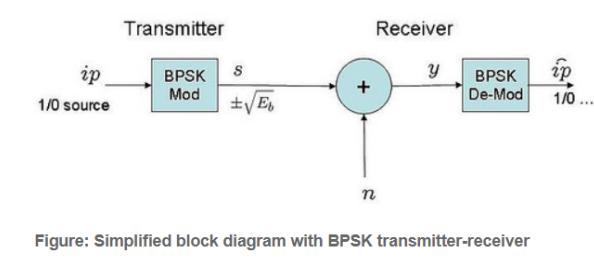
\includegraphics[scale=.5]{Img/Gausodo1.png}
\end{center}
\subsection{Thêm nhiễu Gaussian vào dạng sóng truyền đi}
\textbf{a) Khi sóng truyền có dạng} r(t) = s(t) + n(t), 0 ≤ t ≤ Tb.
\begin{center}
     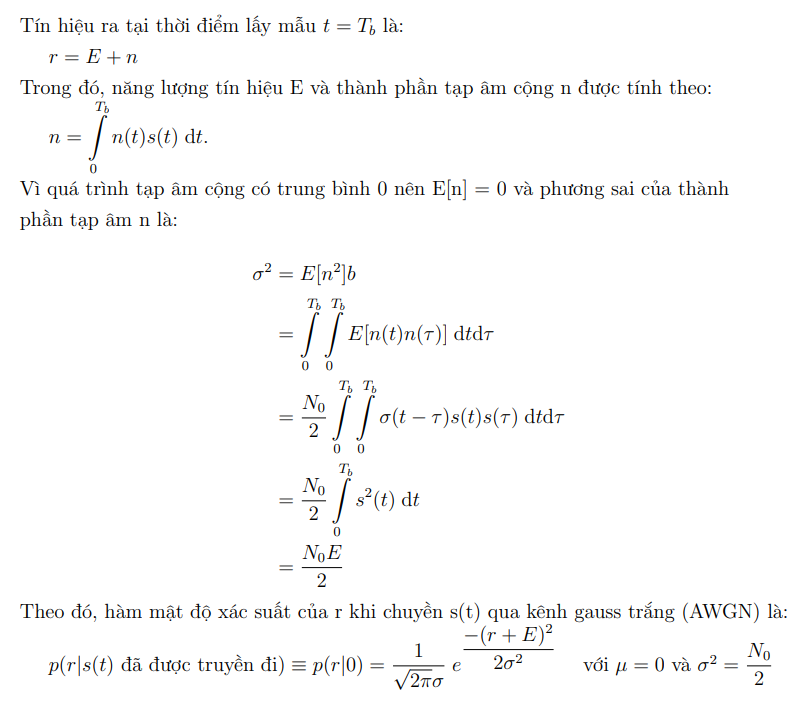
\includegraphics[scale=.6]{Img/tichphannangluong.png}
\end{center}
\begin{center}
     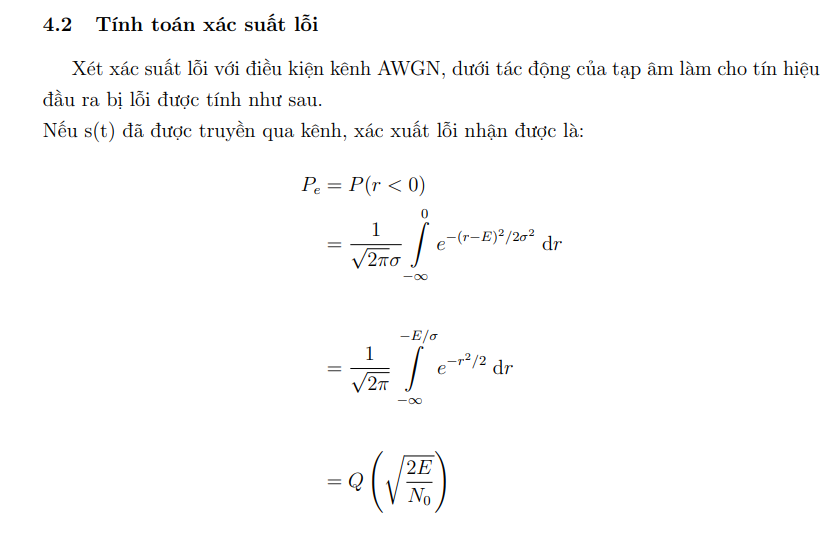
\includegraphics[scale=.7]{Img/tinhtoanxacsuatloi.png}
\end{center}
\newpage
\subsection{Mã nguồn điều chế tín hiệu/ giải điều chế có sự can thiệp bởi nhiễu Gaussian PSK sử dụng ngôn ngữ Python, trình bày Jupyter Notebook }
\textbf{Thêm nhiễu Gaussian với phương sai N0/2, giá trị trung bình = 0}
\begin{lstlisting}
N0 = 2
noise = np.random.normal(0, np.sqrt(N0/2), psk.shape)          
psk_noisy = psk + noise #r(t) = s(t) + n(t)                    
\end{lstlisting}
\textbf{Vẽ tín hiệu khi đã thêm nhiễu nhiệt}
\begin{lstlisting}
fig, ax = plt.subplots(1, 1, figsize=(15, 5))
ax.plot(t, psk_noisy, 'r')
ax.set_title('Tin hieu PSK, nhieu Gaussian')
ax.set_xlabel('t---->')
ax.set_ylabel('Gia tri')
plt.show()
\end{lstlisting}
\begin{center}
     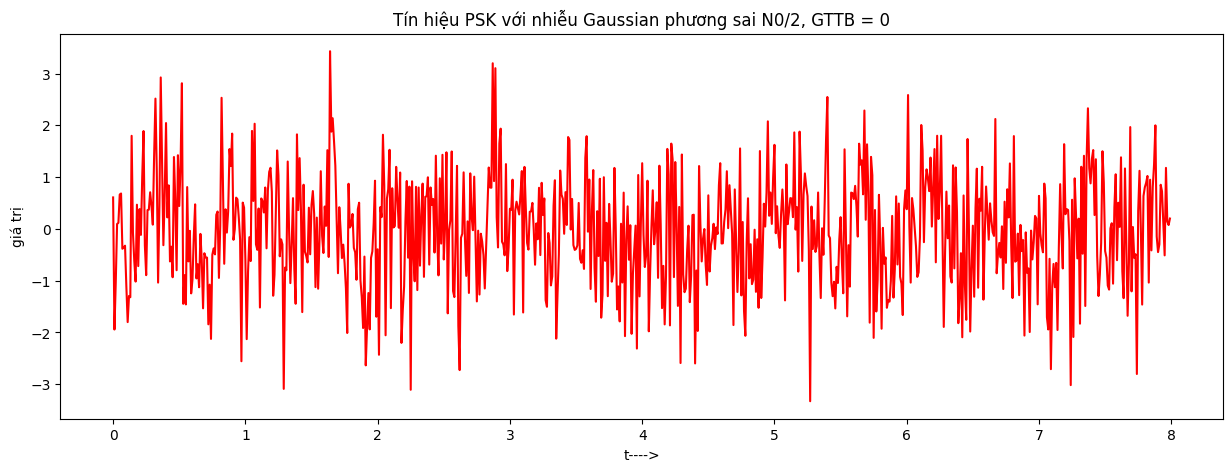
\includegraphics[scale=.5]{Img/venhieu.png}
\end{center}
\newpage
\textbf{Giải nhiễm Gaussian}
\begin{lstlisting}
def gaussian_noise_cancellation(signal, 
                        cutoff=0.05, order=5):        
    b, a = butter(order, cutoff, btype='low', analog=False)            
    filtered_signal = filtfilt(b, a, signal)                           
    return filtered_signal                                  
\end{lstlisting}
\textbf{Vẽ tín hiệu sau khi giải nhiễu}
\begin{center}
     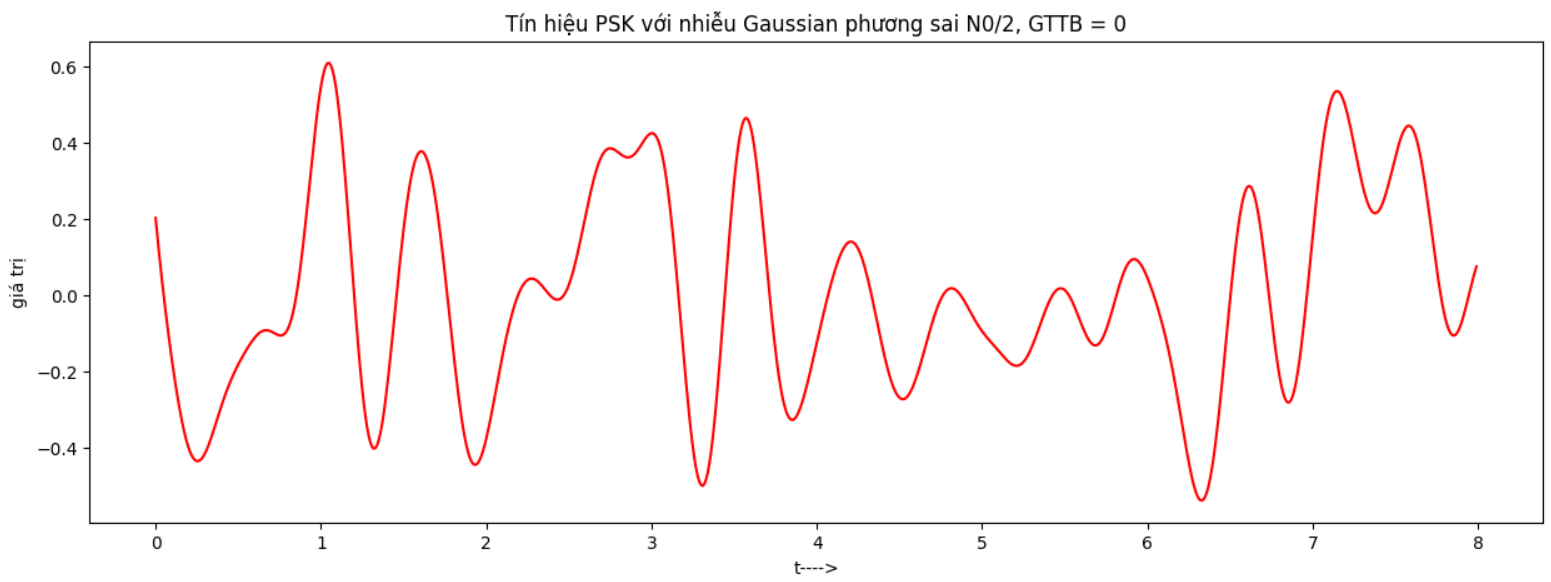
\includegraphics[scale=.5]{Img/giainhieu.png}
\end{center}
\newpage
\section{Tính xác suất lỗi bit của kênh Gaussian PSK}
\subsection{Xác suất lỗi bit theo lí thuyết}
\begin{center}
     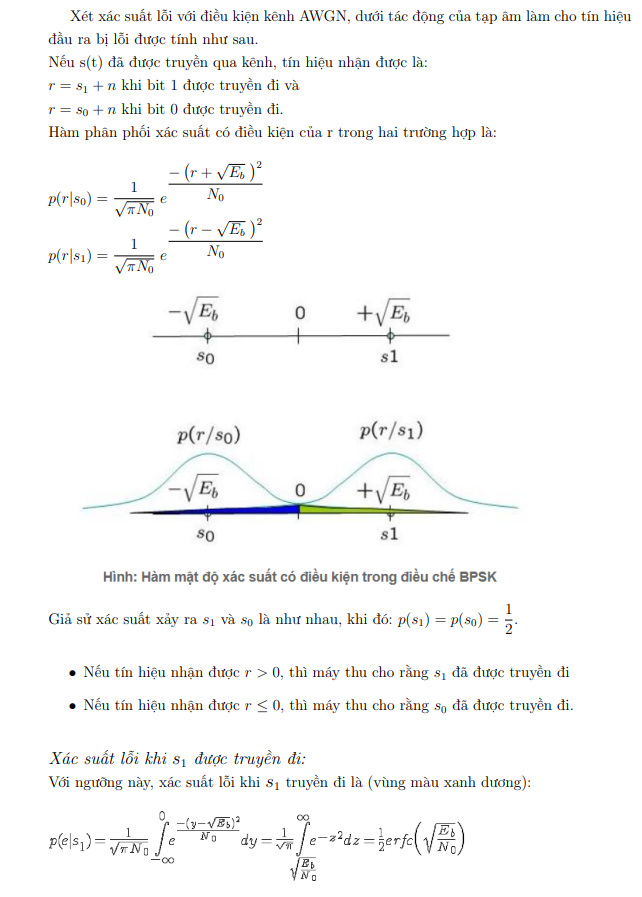
\includegraphics[scale=1]{Img/tinhxacsuatloibitkenhGau.png}
\end{center}
\newpage
\begin{center}
     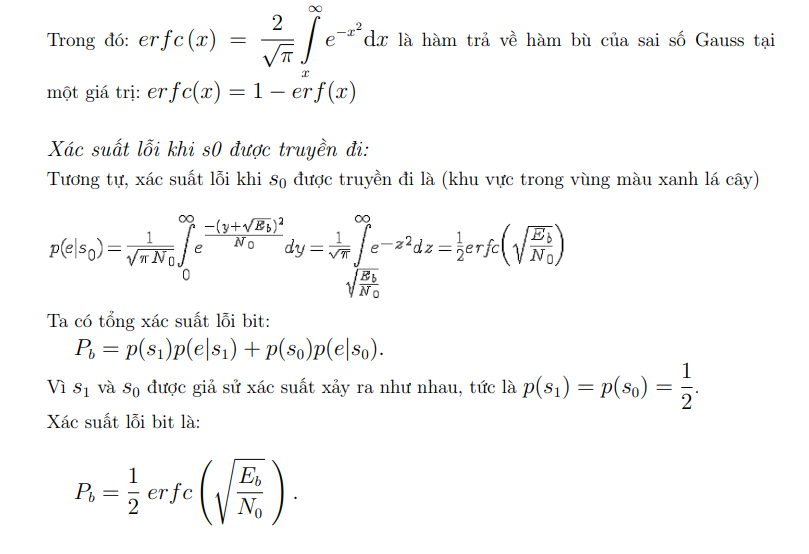
\includegraphics[scale=.8]{Img/tinhxacsuatloibitkenhGau2.png}
\end{center}
\newpage
\subsection{Mã nguồn tính xác suất lỗi bit}
\begin{lstlisting}
    def calculate_bit_error_rate(bitBanDau, bitNhanDuoc):
    num_errors = 0
    for i in range(len(bitBanDau)):
        if bitBanDau[i] != bitNhanDuoc[i]:
            num_errors += 1
    ber = num_errors / len(bitBanDau)
    return ber
    bitBanDau = m
    bitNhanDuoc = demod
    ber = calculate_bit_error_rate(bitBanDau, bitNhanDuoc)
    print("Xác xuất lỗi bit: {:.2f}%".format(ber * 100))
\end{lstlisting}




\newpage
\newpage

	Phổ biến nhất, kênh không được sử dụng trực tiếp cho việc truyền tải tín hiệu dải gốc. Tín hiệu dải gốc signal được sử dụng để điều khiển một số thông số của sóng nạp, khiến cho các thông số thay đổi theo sự thay đổi của tín hiệu dải gốc, đây là gọi là tín hiệu tần số. Theo nguyên lý, sóng nạp được chỉnh sửa có thể là bất kỳ dạng sóng nào, miễn là nó phù hợp cho việc truyền tải trung gian và có thể phân biệt được giữa các tín hiệu khác nhau. Thực tế, trong hầu hết các hệ thống giao tiếp số, tín hiệu $sin$ là lựa chọn làm sóng nạp, vì nó đơn giản và dễ tạo và nhận. So với tín hiệu tương tự và tín hiệu số, nguyên lý cơ bản là giống nhau, khác biệt chỉ là trong quá trình tín hiệu tương tự, thông số của sóng nạp được chỉnh sửa liên tục, tại đầu nhận, các thông số của sóng nạp được đánh giá liên tục.


\section{Cơ sở lí thuyết}

    Khi tín hiệu dữ liệu số được truyền bằng phương pháp FM, thì kỹ thuật này được gọi là kỹ thuật dời tần (FSK: Frequency- Shift Keying). Nó được sử dụng rộng rãi vì khả năng chống lại sự mất tầm rất mạnh. FSK được sử dụng để truyền tín hiệu kỹ thuật số với các tần số khác nhau, và tần số của tín hiệu nạp được điều khiển bởi tín hiệu kỹ thuật số cơ sở. Tín hiệu nạp được nhận tại đầu nhận được chuyển đổi thành tín hiệu kỹ thuật số để hoàn thành quá trình truyền thông thông tin. 2FSK là hình thức đơn giản nhất của chuyển dấu chuyển tần số, có thể biểu diễn như sau: \\
	\[S(t) = m_1(t)A\cos(2 \pi f_1 t + \varphi _1) + m_2(t)A\cos(2 \pi f_2 t + \varphi _2) \] \\
	
Mô hình điều chế đa tần số có thể được hình thành bằng cách thêm sóng hình sin với các số khác nhau,tần số và biên độ khác nhau. Ví dụ: \\
	\[ S(t) = 
\begin{array}{cc}
m_1(t)A\cos(2 \pi f_1 t + \varphi _1) & + \\
m_2(t)A\cos(2 \pi f_2 t + \varphi _2) & + \\
m_3(t)A\cos(2 \pi f_3 t + \varphi _3) & + \\
 & \vdots \\
m_m(t)A\cos(2 \pi f_m t + \varphi _m) & +
\end{array}
 \] \\
\subsection{Điều chế}
    Phương pháp điều chế 2-FSK sử dụng các tần số khác nhau của sóng mang để biểu diễn các bit khác nhau (0 hoặc 1) của tín hiệu nhị phân cần mã hóa, nói theo cách khác, sóng tín hiệu truyền đi được tạo ra bằng cách thay đổi tần số của sóng mang.\\
Ta có không gian tín hiệu M:
\[ s_1 = \sqrt{\frac{2}{Tb}} cos(2 \pi f_1 t) \]
\[ s_2 = \sqrt{\frac{2}{Tb}} cos(2 \pi f_2 t) \]

Ta có $f_0 = 1/R_b$. Giải sử sóng mang có cần tần số $f_1, f_2 = kf_0$ , $( k \in Z)$.\\
Ta gán: \\
\begin{itemize}
\item Với giá trị bit $1$ : $\sqrt{\frac{2}{Tb}} cos(2 \pi f_1 t)$
\item Với giá trị bit $0$ : $\sqrt{\frac{2}{Tb}} cos(2 \pi f_2 t)$
\end{itemize}
	
\begin{center}
    \begin{figure}[htp]
    \begin{center}
     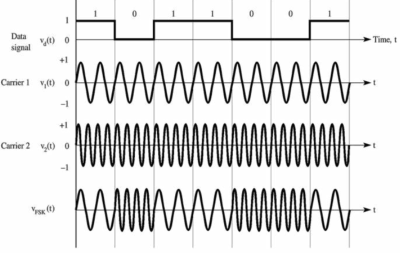
\includegraphics[scale=1]{Img/dieu_che_fsk.png}
    \end{center}
    \caption{Sơ đồ điều chế FSK}
    \label{refhinh1}
    \end{figure}
\end{center}


\subsection{Bộ lọc phối hợp Matched Filter}

Mỗi bộ lọc được đặc trưng bởi đáp ứng xung: $h(t)$ \\
Tín hiệu đầu ra $y(t)$ được xác định bởi tín hiệu đầu vào $x(t)$ và đáp ứng xung như sau:
\[ y(t) = \displaystyle \int_{-\infty}^{\infty} x(\tau)h(t - \tau) d \tau  \]
Theo bài ra ta có: \\
\begin{itemize}
\item Tín hiệu đầu vào là tín hiệu nhận được sau khi điều chế: $p(t)$
\item Đáp ứng xung là $h(t) = b_j(T-t)$
\end{itemize}


Từ đó ta thu được đầu ra của bộ lọc là:
\[ y(t) = \displaystyle \int_{-\infty}^{\infty} p(\tau)h(t - \tau) d \tau =   \displaystyle \int_{-\infty}^{\infty} p(\tau)b_j(T - t + \tau) d \tau \]
Giả thiết lấy mẫu tín hiệu đầu ra tại thời điểm $t = T$
\[ y(t=T) = \displaystyle \int_{-\infty}^{\infty} p(\tau)b_j(\tau) d \tau =  \displaystyle \int_{0}^{T} p(\tau)b_j(\tau) d \tau = p_j\]
\begin{center}
    \begin{figure}[htp]
    \begin{center}
     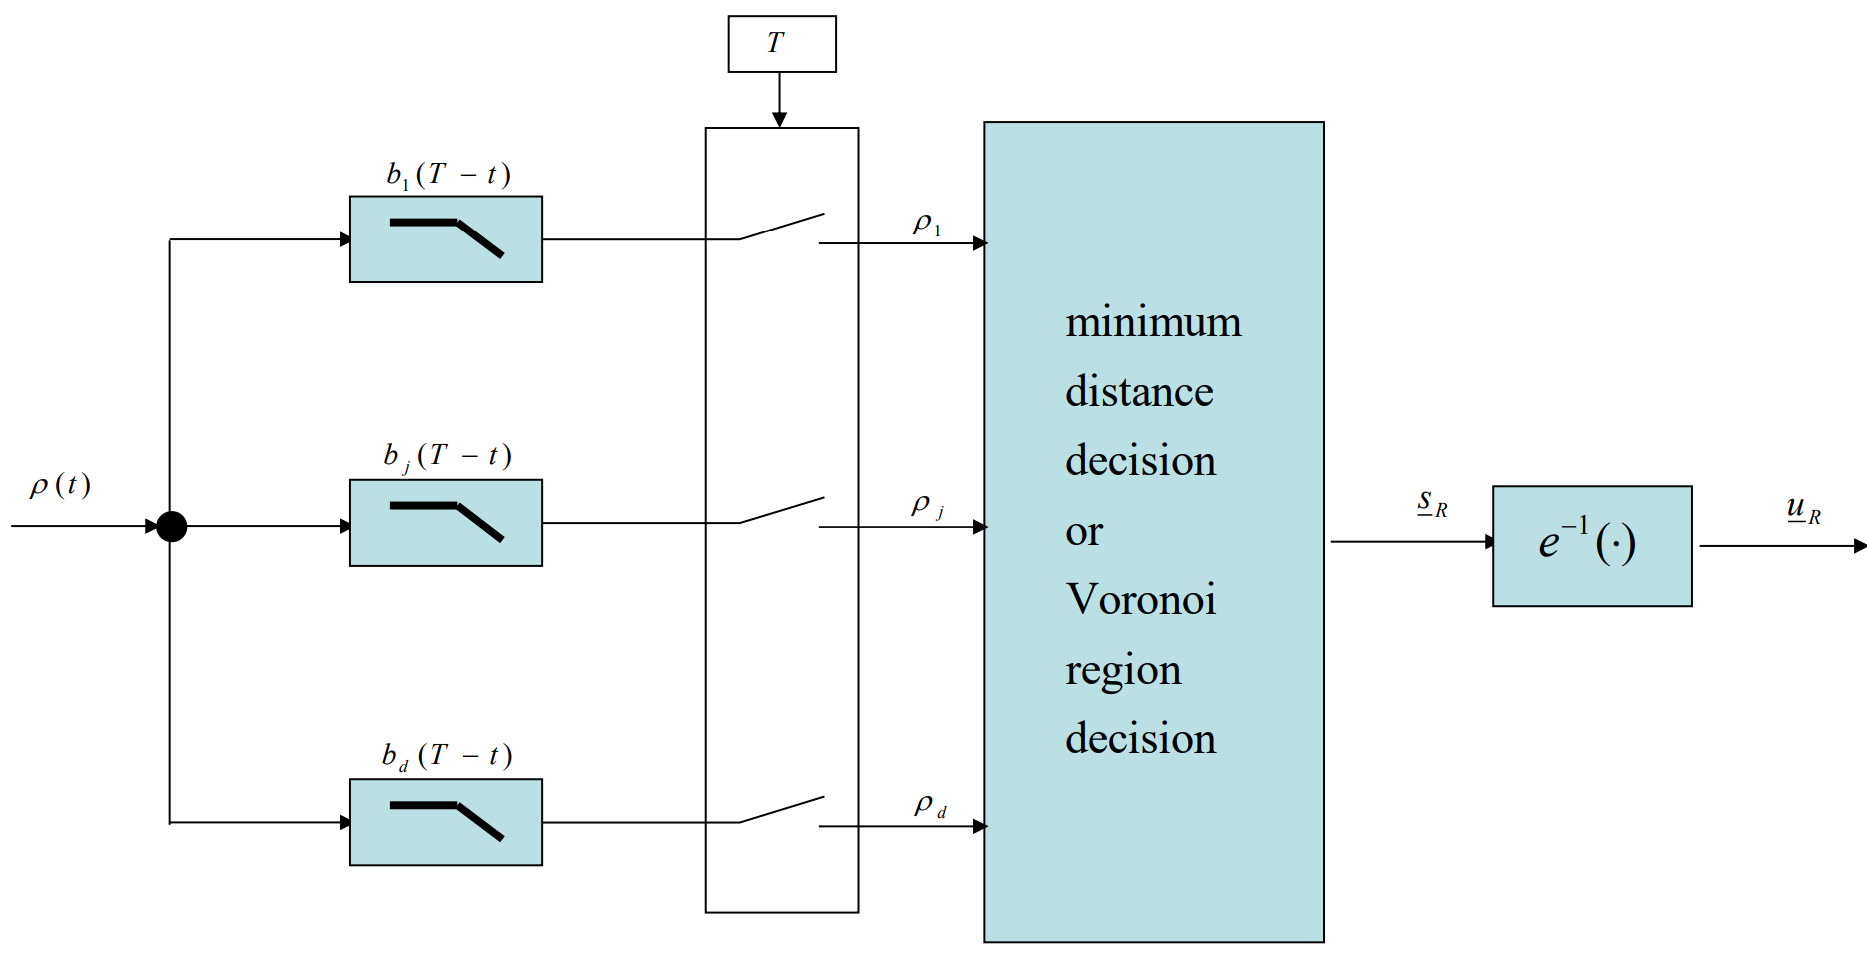
\includegraphics[width=\textwidth]{Img/MF.png}
    \end{center}
    \end{figure}
\end{center}
\subsection{Nguyên lí giải điều chế}
Các bước giải điều chế FSK:
\begin{enumerate}
\item Từ M xây dựng cơ sở trực chuẩn:
\[ b_1(t) = \sqrt{\frac{2}{T}} P_T(t)cos(2 \pi f_1 t) \]
\[ b_2(t) = \sqrt{\frac{2}{T}} P_T(t)cos(2 \pi f_2 t) \]
\item Xây dựng bộ lọc phối hợp Matched Filter (MF)
\item Xác định giá trị đầu ra của bộ lọc tại các thời điểm $t = nT$
\item Tính khoảng cách đến các điểm $s_1$, $s_2$ được biểu diễn trong hệ trục tọa độ trực chuẩn. Nếu khoảng cách nào nhỏ nhất thì quyết định sóng mang này biểu diễn bit nào.



\end{enumerate}


\section{Lập trình với python}
\subsection{Tạo chuỗi bit ngẫu nhiên và tín hiệu xung}
Tạo chuỗi N bit ngẫu nhiên bằng hàm $rantint$ trong python và biểu diễn dưới dạng xung vuông:

\begin{lstlisting}
import random
import numpy as np
import matplotlib.pyplot as plt

def random_bits_array(n):   
    return [random.randint(0, 1) for _ in range(n)]
def message_signal(m,T):  
    t = np.arange(0, T, T/100)
    message = []
    not_message = []
    for i in range(len(m)):
        
        if m[i] == 1:
            m_s = np.ones(len(t))
            invm_s = np.zeros(len(t))
        else:
            m_s = np.zeros(len(t))
            invm_s = np.ones(len(t))
        message.extend(m_s)
        not_message.extend(invm_s)
    return message , not_message
           
N = 8       
Tb = 1       
T = 1*N    
t = np.arange(0, T, T/800)

m = random_bits_array(N)

fig, ax = plt.subplots(2, 1, figsize=(15, 5))
fig.subplots_adjust(hspace=0.5)
ax[0].stem(m)
ax[0].set_title('binary data')
ax[0].set_xlabel('n---->')
ax[0].set_ylabel('b(n)')
message , not_message = message_signal(m,T)
print(len(message), len(not_message))
ax[1].plot(t,message, 'r')
ax[1].set_title('message signal-1')
ax[1].set_xlabel('t---->')
ax[1].set_ylabel('c1(t)')

\end{lstlisting}


\begin{center}
    \begin{figure}[htp]
    \begin{center}
     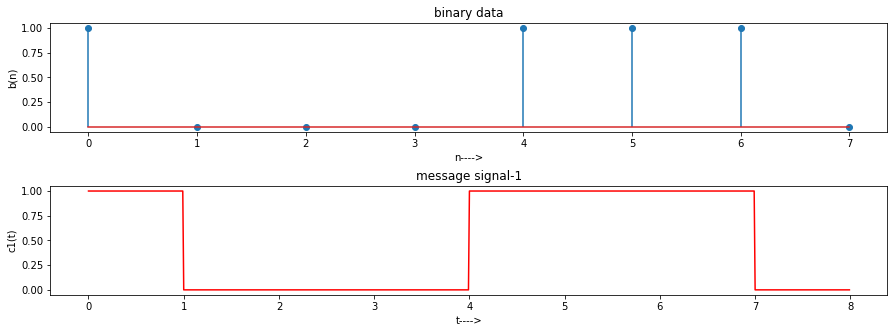
\includegraphics[scale=.5]{Img/binary_signal.png}
    \end{center}
    \caption{Tín hiệu bit và tín hiệu xung}
    \label{refhinh1}
    \end{figure}
\end{center}

\subsection{Tạo tín hiệu sóng mang}
Tạo hai sóng mang cho các tín hiệu tương ứng
\begin{itemize}
\item Với giá trị bit $1$ : $\sqrt{\frac{2}{Tb}} cos(2 \pi f_1 t)$
\item Với giá trị bit $0$ : $\sqrt{\frac{2}{Tb}} cos(2 \pi f_2 t)$
\end{itemize}
\begin{lstlisting}
fc1 = 5
fc2 = 10
c1 = np.sqrt(2/Tb) * np.sin(2 * np.pi * fc1 * t)
c2 = np.sqrt(2/Tb) * np.sin(2 * np.pi * fc2 * t)
fig, ax = plt.subplots(2, 1, figsize=(15, 5))
fig.subplots_adjust(hspace=0.5)
ax[0].plot(t, c1)
ax[0].set_title('carrier signal-1')
ax[0].set_xlabel('t---->')
ax[0].set_ylabel('c1(t)')

ax[1].plot(t, c2)
ax[1].set_title('carrier signal-2')
ax[1].set_xlabel('t---->')
ax[1].set_ylabel('c2(t)')
\end{lstlisting}

\begin{center}
    \begin{figure}[htp]
    \begin{center}
     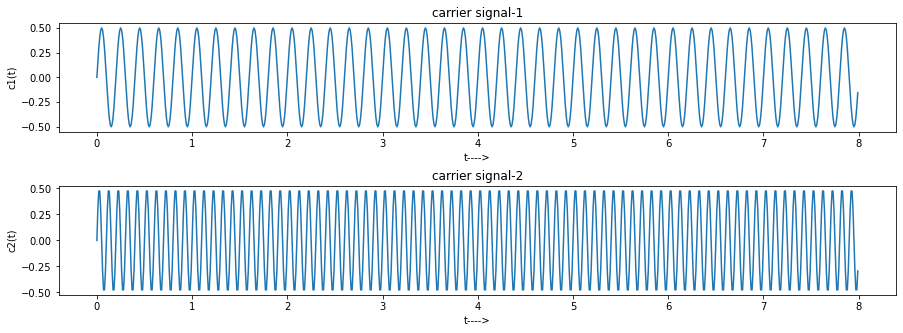
\includegraphics[scale=.5]{Img/carrier_signal.png}
    \end{center}
    \caption{Tín hiệu sóng mang}
    \label{refhinh1}
    \end{figure}
\end{center}

\subsection{Tín kiệu điều chế FSK}
Gán tín hiệu với bit tương ứng. Bit $1$ có tần số $f_1$, bit $0$ có tần số $f_2$.
Gán fsk là mảng chứa giá trị của tín hiệu sau khi điều chế
\begin{lstlisting}
fig, ax = plt.subplots(1, 1, figsize=(15, 3))
def modulation(message_signal,not_message_signal):  
    return message_signal*c1+ not_message*c2
fsk = modulation(message,not_message)
ax.figsize=(15, 5)
ax.plot(t,fsk, 'b')
ax.set_title('FSK signal')
ax.set_xlabel('t---->')
ax.set_ylabel('FSK')
\end{lstlisting}


\begin{center}
    \begin{figure}[htp]
    \begin{center}
     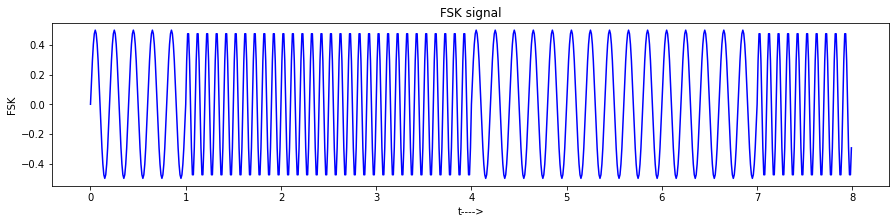
\includegraphics[scale=.5]{Img/modulation.png}
    \end{center}
    \caption{Tín hiệu điều chế}
    \label{refhinh1}
    \end{figure}
\end{center}

\subsection{Giải điều chế}
	
	
\begin{lstlisting}
fig, ax = plt.subplots(1, 1, figsize=(15, 3))
def demodulation(fsk,N):
    start = 0
    end = 99
    demod = np.zeros(N)
    for i in range(N):
        x1 = np.sum(c1[start:end] * fsk[start:end])
        x2 = np.sum(c2[start:end] * fsk[start:end])
        x = x1 - x2
        if x > 0:
            demod[i] = 1
        else:
            demod[i] = 0
        start += 100
        end += 100
    return demod
demod = demodulation(fsk,N)
ax.stem(demod)
ax.set_title("Demodulated data")
ax.set_xlabel("n---->")
ax.set_ylabel("b(n)")
\end{lstlisting}

\begin{center}
    \begin{figure}[htp]
    \begin{center}
     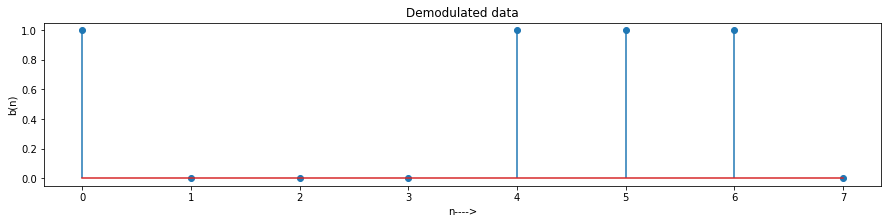
\includegraphics[scale=.5]{Img/demodulation}
    \end{center}
    \caption{Giải điều chế}
    \label{refhinh1}
    \end{figure}
\end{center}

\subsection{Điều chế và giải điều chế FSK dưới tác động của nhiễu Gausian}
Dùng hàm random.random trong python để tạo phân bố chuẩn Gauss
\begin{lstlisting}
def white_noise(rho, sr, n, mu=0):
    sigma = rho * np.sqrt(sr/2)
    noise = np.random.normal(mu, sigma, n)
    return noise
gauss = fsk + white_noise(1,1,800)
fig, ax = plt.subplots(1, 1, figsize=(15, 5))
ax.plot(gauss, 'b')
ax.set_title('FSK signal')
ax.set_xlabel('t---->')
ax.set_ylabel('FSK')

\end{lstlisting}
\begin{center}
    \begin{figure}[htp]
    \begin{center}
     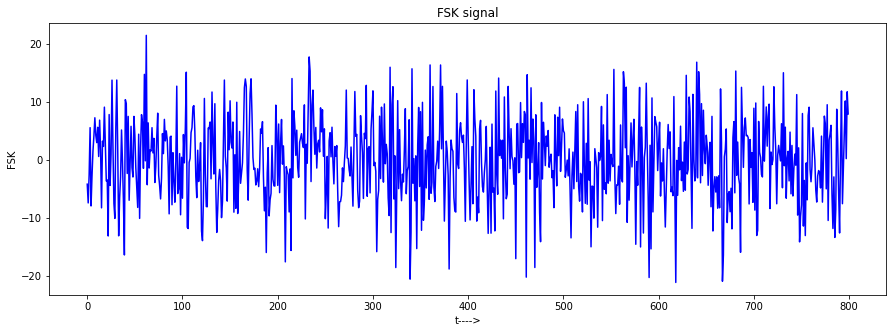
\includegraphics[scale=.5]{Img/add_gauss_signal.png}
    \end{center}
    \caption{Tín hiệu thêm nhiễu Gauss}
    \label{refhinh1}
    \end{figure}
\end{center}
\newpage
\section{Tính xác suất lỗi bit}
Chiếu hai tín hiệu nên không gian trực chuẩn ta có:
\[ M = \{ s_1(1,0), s_2(0,1) \} \]
Từ đó ta có vùng Voronoi được định nghĩa như sau:
\[ V(s_1) = \{  p = (p_1,p_2), p_1 \ge p_2 \} \]
\[ V(s_2) = \{  p = (p_1,p_2), p_2>p_1 \} \]
Ta có:
\begin{equation}
	P_s(e) = \frac{1}{2} (P_s(e|s_T = s1) + P_s(e|s_T = s_2)  
\end{equation}
 
Ta cần tính:
\[  P_s(e|s_T = s_1) = P(p \in s_2 | s_T = s_1) = P(p_2 > p_1 | s_T = s_1)\]
Mà $ p_1 = s_1 + n_1 $, $ p_2 = s_2 + n_2  $ và $s_1 = s_2 = 1$ suy ra:
\[ P_s(e|s_T = s_1) = P(n_2 > n_1) = P(n_2 - n_1 > 0)\]
\[ \rightarrow P_s(e|s_T = s_1) = \frac{1}{2} erfc(0) \]
Tương tụ ta có 
$P_s(e|s_T = s_2) = \frac{1}{2} erfc(0) $ \\
Thay vào (1) ta có $P_s(e) = \frac{1}{2} erfc(0)$

Vậy xác suất lỗi bit trong AWGN là: $P_s(e) = \frac{1}{2} erfc(0)$

\newpage
\section{Trích Nguồn}
1)  Tạ Hải Tùng, Slide Nhập môn Kỹ thuật Truyền thông. 2018. \\
2)  Mau-Chung Frank Chang’s Lab, "Analysis of Noncoherent ASK ModulationBased RF-Interconnect for Memory Interface" in IEEE Journal on Emerging and Selected Topics in Circuits and Systems.  \\
3) "Digital Communications: Fundamentals and Applications" của Bernard Sklar \\ 
4) "Introduction to Digital Communication" của Rodger E. Ziemer và Roger L. Peterson \\ 
5) "Principles of Digital Communication" của Robert G. Gallager \\ 
6) "Digital Communication" của Simon Haykin \\
7) "Communication Systems Engineering" của John G. Proakis và Masoud Salehi \\ 
3) 
\end{document}
\end{document}